
In the last three Chapters we have introduced six important \PETSc types (object classes).  All are important for solving PDEs:

\medskip
\begin{tabular}{ll}
Chapter \ref{chap:ls}: \pVec, \pMat, \pKSP, \pPC \hspace{.5in} & for linear algebra \\
Chapter \ref{chap:st}: \pDMDA                    & for structured grids \\
Chapter \ref{chap:nl}: \pSNES                    & for Newton's method
\end{tabular}

\bigskip

Each example in the rest of the book will use \pVec, \pMat, \pKSP, \pPC, and \pSNES objects.  From now on we will even solve linear PDEs using a \pSNES object, for example in Chapter \ref{chap:ad}.  (In such cases we know that one Newton iteration suffices in theory.)  Always using \pSNES allows uniform code structure and more flexibility when it comes to changing the PDE problem.

Though new ideas appear in it, the current Chapter takes a break from introducing new \PETSc types.  Instead we look at a PDE which arises from minimization in a function space, and we introduce a structured-grid finite element method.  This example is a nonlinear Poisson-like equation with solution-dependent diffusivity.

The example code here is the last one shown in full.  In later Chapters we show snippets.  The reader can always examine and run the complete codes by looking in the \texttt{c/} directory of the \texttt{p4pdes} repository.


\section{$p$-Laplacian equation as minimization}

Let $\Omega$ be a domain (connected open subset) in $\RR^2$ with well-behaved boundary.\sidenote{A Lipschitz boundary will suffice in theory.  In practice we use polygonal domains, namely a rectangle in the current Chapter and general polygons in Chapter \ref{chap:un}.}  For simplicity, noting our numerical method will use the point values of this function, suppose $f\in C(\overline \Omega)$ is given.  Consider this nonlinear functional for $p \ge 1$,
\begin{equation}
    I[u] = \int_\Omega \frac{1}{p} |\grad u|^p - fu.  \label{eq:of:functional}
\end{equation}
This functional is well-defined and continuous on the Sobolev space \citep{AdamsFournier2003,Evans2010} of integrable functions on $\Omega$ which have integrable gradient,
\begin{equation}
    W^{1,p}(\Omega) = \left\{w \,:\, \int_\Omega |w|^p < \infty \,\, \& \, \int_\Omega |\grad w|^p < \infty\right\}, \label{eq:of:sobolevdefn}
\end{equation}
a Banach space with norm $\|w\|_{W^{1,p}} = \left(\int_\Omega |w|^p + \int_\Omega |\grad w|^p\right)^{1/p}$.

\begin{marginfigure}
\includegraphics[width=1.2\textwidth]{figs/minsurf} % generated by figs/minsurf.tex
\medskip
\caption{The functional $I[u]$ is analogous to the convex surface $z = \tfrac{1}{4}(x^4 + y^4) - 2x + 2y$ shown here, but with input from the $\infty$-dimensional space $W_g^{1,p}(\Omega)$ instead of the plane $\RR^2$.}
\label{fig:of:cartoonfunctional}
\end{marginfigure}

The reader may visualize $I[u]$ in cartoon form as in Figure \ref{fig:of:cartoonfunctional}.  As suggested by the cartoon, this functional has a unique minimum, at least once we add boundary conditions.

We add Dirichlet conditions (Chapter \ref{chap:st}) by choosing a real-valued function $g$, defined along $\partial \Omega$, so as to determine an affine subspace of $W^{1,p}(\Omega)$, namely
\begin{equation}
    W_g^{1,p}(\Omega) = \left\{w \,:\, w \in W^{1,p}(\Omega) \,\, \& \,\, w\big|_{\partial \Omega} = g\right\}.  \label{eq:of:affinedirichlet}
\end{equation}
For this to make sense one might require $g \in L^p(\partial \Omega)$ and note that the equation $w\big|_{\partial \Omega} = g$ has a precise ``trace operator'' meaning \citep[section 5.5]{Evans2010}.  Again, however, because our numerical scheme will use the point values of $g$, we assume $g\in C(\partial\Omega)$.  These considerations also define a vector subspace $W_0^{1,p}(\Omega) \subset W^{1,p}(\Omega)$, in the case where $g=0$, which we will use for ``test'' functions below.

The functional $I[u]$ has two significant properties.  First, $I[u]$ is \emph{coercive} in the sense that if the input function is large in norm then the output is large:
\begin{equation}
\lim_{\|u\|_{W^{1,p}} \to +\infty} I[u] = +\infty.   \label{eq:of:coercivity}
\end{equation}
Second it is \emph{convex}, meaning that
\begin{equation}
I[\lambda u + (1-\lambda) v] \le \lambda I[u] + (1-\lambda) I[v]    \label{eq:of:convexity}
\end{equation}
if $u,v\in W_g^{1,p}(\Omega)$ and $0 \le \lambda \le 1$.  We say $I[u]$ is \emph{strictly convex} if $\|u-v\|_{W^{1,p}} > 0$ and $0 < \lambda < 1$ implies strict inequality in \eqref{eq:of:convexity}.  These two properties of $I[u]$, coercivity and convexity, are addressed in Exercise \ref{chap:of}.\ref{exer:of:twoproperties}.

A standard theorem in the calculus of variations \citep[Theorem 8.2.2]{Evans2010} shows that the coercivity and strict convexity of $I[u]$ suffice to imply that the problem
\begin{equation}
\min_{u \in W_g^{1,p}(\Omega)} I[u] \label{eq:of:plapmin}
\end{equation}
has a unique solution.  Strict convexity is used to show uniqueness, but convexity also implies that $I[u]$ is continuous enough to have a minimum on compact sets in the appropriate topology.\sidenote{Namely $I[u]$ is \emph{weakly lower semi-continuous}. This means, by definition, that $\liminf_{v\rightharpoonup u} I[v] \ge I[u]$, using the weak topology on $W^{1,p}(\Omega)$ \citep[section 8.2]{Evans2010}.}  Compactness arises from coercivity in the sense that bounded, closed subsets of $W^{1,p}(\Omega)$, which arise in the existence proof as sets $\{w\,:\,I[w] \le L\}$, are compact in the weak topology.

Being good calculus students we seek the solution to minimization problem \eqref{eq:of:plapmin} by taking the derivative (gradient) and setting it to zero.  If $p>1$ then the functional $I[u]$ is smooth enough to have a gradient, as we show next.  The solution of minimization \eqref{eq:of:plapmin} is then also the solution to a nonlinear equation.

Assume $\eps\in \RR$ and $u,v \in W^{1,p}(\Omega)$.  Then, by the binomial theorem,
\begin{align*}
I[u+\eps v] - I[u] &= \int_\Omega \frac{1}{p} |\grad u + \eps \grad v|^p - \frac{1}{p} |\grad u|^p - \eps f v \\
   &= \eps \left(\int_\Omega |\grad u|^{p-2} \grad u \cdot \grad v - f v\right) + O(\eps^2).
\end{align*}
Thus the directional derivative exists and has this formula:
\begin{equation}
\grad I[u](v) = \lim_{\eps\to 0} \frac{I[u+\eps v] - I[u]}{\eps} = \int_\Omega |\grad u|^{p-2} \grad u \cdot \grad v - f v. \label{eq:of:plapfunctionalderivative}
\end{equation}
That is, for each $u \in W^{1,p}(\Omega)$, formula \eqref{eq:of:plapfunctionalderivative} defines a linear and continuous map, the gradient
   $$\grad I[u] : W^{1,p}(\Omega) \to \RR.$$

If $u \in W_g^{1,p}(\Omega)$ and $v\in W_0^{1,p}(\Omega)$ then $u+\eps v\in W_g^{1,p}(\Omega)$.  Thus if $u \in W_g^{1,p}(\Omega)$ solves \eqref{eq:of:plapmin} then the above calculation also shows $\grad I[u](v)=0$ or
\begin{equation}
\int_\Omega |\grad u|^{p-2} \grad u \cdot \grad v - f v = 0 \label{eq:of:plapweakform}
\end{equation}
for all $v\in W_0^{1,p}(\Omega)$.  Note that the test functions $v$ have zero boundary values in this calculation.  We refer to \eqref{eq:of:plapweakform} as the \emph{weak form} of the $p$-\emph{Laplacian} equation.\sidenote{Alternate names include \emph{variational equation} and \emph{Euler-Lagrange equation}.}

If the solution $u \in W_g^{1,p}(\Omega)$ to problem \eqref{eq:of:plapmin} or equation \eqref{eq:of:plapweakform} is actually smooth enough to have continuous second derivatives\sidenote{\emph{Proving} this much smoothness is possible in some cases when the domain $\Omega$ and data $f,g$ are well-behaved, but beyond our scope.} then we can derive the \emph{strong form} PDE \eqref{eq:of:plapstrongform} below, as follows.  An integration-by-parts \citep[Appendix C]{Evans2010} gives
    $$-\int_\Omega \Div\left(|\grad u|^{p-2} \grad u\right) v - \int_\Omega f v + \int_{\partial \Omega} v |\grad u|^{p-2} \grad u \cdot \bn = 0.$$
The boundary integral is zero because $v\in W_0^{1,p}(\Omega)$.  It follows that
\begin{equation}
- \Div\left(|\grad u|^{p-2} \grad u\right) = f.
\label{eq:of:plapstrongform}
\end{equation}
This is the traditional form of the $p$-Laplacian equation, and it reduces to the Poisson equation \eqref{poissonsquare} if $p=2$.

Before proceeding to a numerical solution, the main ideas of the above theory are simple and worth restating:
\begin{quote}
Minimization problem \eqref{eq:of:plapmin} is equivalent to the weak form \eqref{eq:of:plapweakform}.  These become the strong form \eqref{eq:of:plapstrongform} when the solution $u$ is smooth.  Thus the $p$-Laplacian equation arises from minimization.
\end{quote}

It is also worthwhile pausing to choose a particular test problem.  We want a problem for which we know the exact solution, and an easy choice is to ``manufacture'' a test problem by starting with a simple solution:
\begin{equation}
    u(x,y) = \frac{1}{2} (x+1)^2 (y+1)^2. \label{eq:of:exactsolution}
\end{equation}
This formula also determines $g$ along $\partial \Omega$.  The source function $f$ is then computed by hand\sidenote{The by-hand derivative calculation which generates $f(x,y)$ from the exact solution $u(x,y)$ is acceptably simple, but it is still error-prone.  Because by-hand calculation errors are likely to be un-correlated to code-implementation errors, however, agreement is likely to reflect correctness.} from the strong form \eqref{eq:of:plapstrongform}.

It is an easy exercise to show that the coefficient of the $p$-Laplacian equation is bounded and thus that equation \eqref{eq:of:plapweakform}, or \eqref{eq:of:plapstrongform}, is uniformly elliptic \citep{Evans2010} at the solution \eqref{eq:of:exactsolution}:
\begin{equation}
0 < 2^{(p-2)/2} \le |\grad u|^{p-2} \le 2^{7(p-2)/2}.  \label{eq:of:coeffbounds}
\end{equation}
However, though such bounds apply at the solution, they do not necessarily apply to the approximations (iterates) in a numerical procedure.  We might ``lose ellipticity'' on the way to the solution; see Exercise \ref{chap:of}.\ref{exer:of:regularize}.


\section{Structured $Q^1$ finite elements}

Initially we will use \PETSc to numerically solve the $p$-Laplacian equation as minimization problem \eqref{eq:of:plapmin}, based only on code that computes the functional $I[u]$ from a representation of $u \in W_g^{1,p}(\Omega)$.  Thus, once we have a finite-dimensional representation of the input $u$, we need only implement formula \eqref{eq:of:functional} for $I[u]$.

Such a minimization approach may suffice for prototyping, but we will augment it by additional derivative-computing code so that the problem becomes a nonlinear-residual problem like that of Chapter \ref{chap:nl}.  Initially, however, we will ask \PETSc to use finite differences when it needs derivatives (gradients) in minimizing $I[u]$.  In this case the nonlinear equations, and the associated residual functions, are approximate and are internal to \PETSc.

For the representation of $u$ we introduce a structured-grid finite element method (FEM) using quadrilateral elements.  The gridded unknowns, which live on a structured grid somewhat different from that in Chapter \ref{chap:st}, now represent an element of a function space.

\begin{figure}
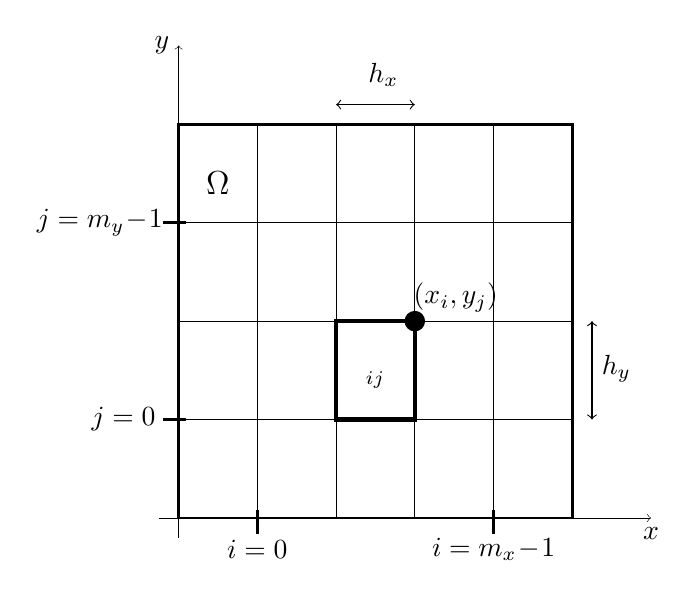
\begin{tikzpicture}[scale=5.0]
  % axes
  \draw[->,very thin] (-0.05,0.0) -- (1.2,0.0) node[below] {$x$};
  \draw[->,very thin] (0.0,-0.05) -- (0.0,1.2) node[left] {$y$};
  % grid
  \draw[line width=1.0pt] (0.0,0.0) -- (0.0,1.0) -- (1.0,1.0) -- (1.0,0.0) -- cycle;
  \pgfmathsetmacro\fifth{1.0/5.0}
  \pgfmathsetmacro\fourth{1.0/4.0}
  \draw[xstep=\fifth,ystep=\fourth,black,thin] (0.0,0.0) grid (1.0,1.0);
  \node at (0.1,0.85) {\large $\Omega$};
  % outline an element, showing location and dimensions
  \draw[line width=1.5pt] (0.6,0.5) -- (0.4,0.5) -- (0.4,0.25) -- (0.6,0.25) -- cycle;
  \node at (0.5,0.35) {$\square_{ij}$};
  \filldraw (0.6,0.5) circle (0.7pt) node[xshift=5.2mm,yshift=3mm] {$(x_i,y_j)$};
  \draw[<->] (0.4,1.05) -- (0.6,1.05) node[above,yshift=1mm,xshift=-4mm] {$h_x$};
  \draw[<->] (1.05,0.25) -- (1.05,0.5) node[right,yshift=-6mm] {$h_y$};
  % tick marks for i
  \draw[line width=1.0pt] (0.2,-0.04) -- (0.2,0.02);
  \draw[line width=1.0pt] (0.8,-0.04) -- (0.8,0.02);
  \node[yshift=-4mm] at (0.2,0.0) {$i=0$};
  \node[yshift=-4mm] at (0.8,0.0) {$i=m_x\!-\!1$};
  % tick marks for j
  \draw[line width=1.0pt] (-0.04,0.25) -- (0.02,0.25);
  \draw[line width=1.0pt] (-0.04,0.75) -- (0.02,0.75);
  \node[xshift=-7mm] at (0.0,0.25) {$j=0$};
  \node[xshift=-10mm] at (0.0,0.75) {$j=m_y\!-\!1$};
\end{tikzpicture}
\medskip

\caption{The structured grid divides the unit square $\Omega$ into elements $\square_{ij}$ of area $h_x h_y$.  There are $m_x\times m_y$ interior nodes (degrees of freedom).  We index elements by their upper-right corners $(x_i,y_j)$.}
\label{fig:of:q1grid}
\end{figure}

For this Chapter let $\Omega$ be the square $(0,1)\times (0,1)$.  Consider the structured grid on $\Omega$ shown in Figure \ref{fig:of:q1grid}.  Let $m_x,m_y$ be positive integers and define $h_x = 1/(m_x+1)$ and $h_y = 1/(m_y+1)$.  The structured grid is
\begin{equation}
x_i = (i+1) h_x, \qquad y_j = (j+1) h_y \label{eq:of:structuredgridindexing}
\end{equation}
for $i=-1,0,\dots,m_x$ and $j=-1,0,\dots,m_y$, giving $\tilde N = (m_x+2)(m_y+2)$ total nodes in the grid.  The $N=m_x\, m_y$ interior nodes are points with $0 \le i \le m_x-1$ and $0 \le j \le m_y-1$.  These interior nodes correspond to the degrees of freedom; the boundary values of $u\in W_g^{1,p}(\Omega)$ come from $g$. 

The grid has $(m_x+1)(m_x+1)$ rectangular \emph{elements}
   $$\square_{ij} = [x_{i-1},x_i] \times [y_{j-1},y_j]$$
for $i=0,\dots,m_x$ and $j=0,\dots,m_y$.  We index the elements by their upper-right corners.

The functional in \eqref{eq:of:functional} can be computed element-by-element,\footnote{Because element boundaries have zero measure and integration is additive.}
\begin{equation}
I[u] = \sum_{i=0}^{m_x} \sum_{j=0}^{m_y} \int_{\square_{ij}} \frac{1}{p} |\grad u|^p - fu  \label{eq:of:sumoverelements}
\end{equation}
Integration over a single element $\square_{ij}$ can be addressed once we represent $f$ and $u$.  A related sum over elements computes an approximation of the weak form \eqref{eq:of:plapweakform}; see \eqref{eq:of:weakformbasis} and \eqref{eq:of:weakformdetail} below.

By showing the grid in Figure \ref{fig:of:q1grid}, and the sum-over-elements formula \eqref{eq:of:sumoverelements}, we have already motivated how we are going to use \PETSc's \pDMDA structured-grid object.\sidenote{Introduced in Chapter \ref{chap:st}.}  We create this object using a \texttt{BOX} stencil and \texttt{GHOSTED} boundaries in each direction, as in this call extracted from Code \ref{code:plapMain}:
\begin{code}
  DMDACreate2d(COMM,
      DM_BOUNDARY_GHOSTED, DM_BOUNDARY_GHOSTED, DMDA_STENCIL_BOX,
      -3,-3,PETSC_DECIDE,PETSC_DECIDE,1,1,NULL,NULL,&(user.da));
\end{code}
(Note we set the grid defaults to $m_x=m_y=3$.)

Thus the ghosted points in a \pVec \texttt{v} derived from the \pDMDA by
\begin{code}
  DMCreateLocalVector(user.da,&v);
\end{code}
can store values at all $\tilde N = (m_x+2)(m_y+2)$ grid points, while a \texttt{Global} \pVec can store the $N=m_x m_y$ degrees of freedom.

On the other hand, how should we approximate a function $w \in W^{1,p}(\Omega)$ in a manner compatible with a structured grid of rectangles?  One simple choice requires that the approximation $w_h$ be bilinear on each element $\square_{ij}$ and continuous on the whole domain $\Omega$.  These requirements determine $w_h(x,y)$ from the nodal values $w_{ij} = w_h(x_i,y_j)$.  Said another way, there is a linear isomorphism between the vector space $\RR^{\tilde N}$, and an $\tilde N$-dimensional linear subspace of $W^{1,p}(\Omega)$, namely
\begin{equation}
S^h = \left\{v \in C(\Omega) \, \Big| \, v|_{\square_{ij}} \text{ is bilinear}\right\}. \label{eq:of:Shdefn}
\end{equation}
Because the elements are quadrilaterals and the polynomial degree is one, $S^h$ is called a $Q^1$ \emph{finite element space} \citep{Elmanetal2005}

The solution $u$ to minimization problem \eqref{eq:of:plapmin} must, however, have the boundary values given by $g$.  We would want $g$ to be continuous and (appropriately) piece-wise linear on $\partial\Omega$, as otherwise its use conflicts with the restrictions which define $S^h$.  In that case, one may show that the functions
\begin{equation}
S_g^h = \left\{v \in S^h \, \Big| \, v|_{\partial \Omega} = g\right\} \label{eq:of:Sghdefn}
\end{equation}
form an (affine) subspace of $W_g^{1,p}(\Omega)$.  Replacing $W_g^{1,p}(\Omega)$ by $S_g^h$ in problem \eqref{eq:of:plapmin} is a \emph{conforming}\sidenote{A ``nonconforming'' version might have $u_h|_{\partial \Omega}$ as the piecewise-linear interpolant of $g$.} $Q^1$ FEM.  Because an element of $S_g^h$ is entirely determined by its values on interior nodes, $S_g^h$ is an $N=m_x m_y$ dimensional affine subspace of $S^h$.


\section{Formulas on one element}

The next step is to describe a bilinear function on a single element $\square_{ij}$, and to thereby build a basis for space $S_g^h$.  We do this by constructing bilinear functions on a \emph{reference element}
    $$\square_\ast = [-1,1]\times[-1,1]$$
in variables $\xi$ and $\eta$, as shown in Figure \ref{fig:of:q1gridandref}.\sidenote{One may easily avoid using the reference element because all elements are congruent rectangles.  We are, however, thinking ahead toward unstructured examples (Chapter \ref{chap:un}).}

If $v(\xi,\eta)$ is bilinear on $\square_\ast$ then $v(\xi,\eta) = a + b\, \xi + c\, \eta + d\, \xi \eta$.  The monomial basis $\{1,\xi,\eta,\xi\eta\}$ is not, however, a convenient one.  Instead, number the vertices (nodes) of $\square_\ast$ as shown in Figure \ref{fig:of:q1gridandref}:
\begin{align}
(\xi_0,\eta_0) &= (+1,+1), \quad (\xi_1,\eta_1) = (-1,+1),    \label{eq:of:refcorners} \\
(\xi_2,\eta_2) &= (-1,-1), \quad (\xi_3,\eta_3) = (+1,-1). \notag
\end{align}
The four functions
\begin{equation}
\chi_\ell(\xi,\eta) = \frac{1}{4} \left(1 + \xi_\ell \xi\right) \left(1 + \eta_\ell \eta\right)  \quad \text{ for } \ell=0,1,2,3 \label{eq:of:chidefn}
\end{equation}
form a basis of bilinear functions on $\square_\ast$.  The nodal values satisfy $\chi_\ell(\xi_{\ell'},\eta_{\ell'}) = \delta_{\ell\ell'}$ so expanding in this basis uses coefficients equal to the nodal values:
\begin{equation}
v(\xi,\eta) = \sum_{\ell=0}^3 v(\xi_\ell,\eta_\ell) \chi_\ell(\xi,\eta). \label{eq:of:bilinearrepresentationref}
\end{equation}

\begin{figure}
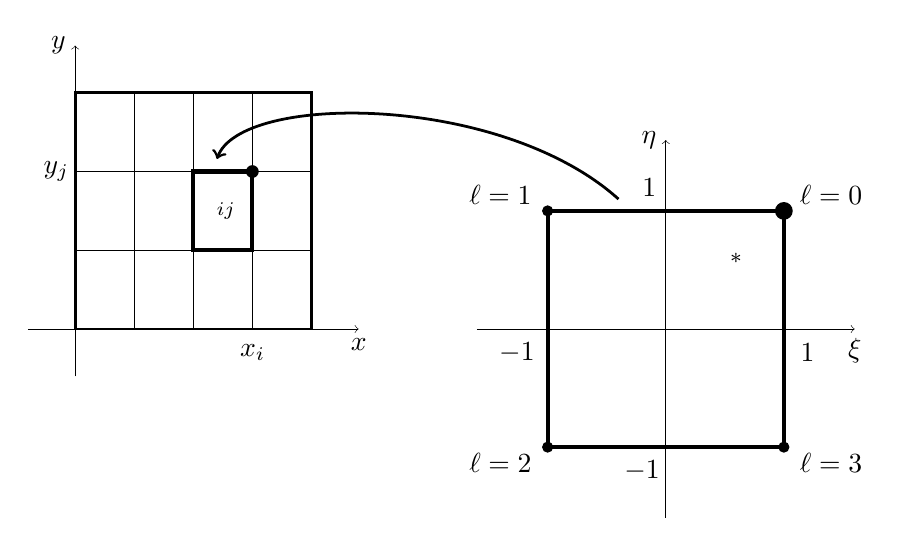
\begin{tikzpicture}[scale=3.0]
% (x,y) elements
  \draw[->,very thin] (-0.2,0.0) -- (1.2,0.0) node[below] {$x$};
  \draw[->,very thin] (0.0,-0.2) -- (0.0,1.2) node[left] {$y$};
  \draw[line width=1.0pt] (0.0,0.0) -- (0.0,1.0) -- (1.0,1.0) -- (1.0,0.0) -- cycle;
  \pgfmathsetmacro\fourth{1.0/4.0}
  \pgfmathsetmacro\third{1.0/3.0}
  \pgfmathsetmacro\twothird{2.0/3.0}
  \draw[xstep=\fourth,ystep=\third,black,thin] (0.0,0.0) grid (1.0,1.0);
  % outline an element
  \draw[line width=1.5pt] (0.5,\third) -- (0.75,\third) -- (0.75,\twothird) -- (0.5,\twothird) -- cycle;
  \node at (0.64,0.5) {$\square_{ij}$};
  \node at (0.751,-0.1) {$x_i$};
  \node at (-0.08,\twothird) {$y_j$};
  \filldraw (0.75,\twothird) circle (0.7pt);

% (xi,eta) reference element
% origin of axes at (2.5,0.0) and square has half-width 0.5
  \draw[->,very thin] (1.7,0.0) -- (3.3,0.0) node[below] {$\xi$};
  \draw[->,very thin] (2.5,-0.8) -- (2.5,0.8) node[left] {$\eta$};
  \draw[line width=1.5pt] (2.0,-0.5) -- (3.0,-0.5) -- (3.0,0.5) -- (2.0,0.5) -- cycle;
  \node at (3.1,-0.1) {$1$};
  \node at (1.87,-0.1) {$-1$};
  \node at (2.43,0.6) {$1$};
  \node at (2.4,-0.6) {$-1$};
  \node at (2.8,0.3) {\large $\square_\ast$};
  \filldraw (3.0,0.5) circle (1.0pt) node[xshift=6mm,yshift=2mm] {$\ell=0$};
  \filldraw (2.0,0.5) circle (0.6pt) node[xshift=-6mm,yshift=2mm] {$\ell=1$};
  \filldraw (2.0,-0.5) circle (0.6pt) node[xshift=-6mm,yshift=-2mm] {$\ell=2$};
  \filldraw (3.0,-0.5) circle (0.6pt) node[xshift=6mm,yshift=-2mm] {$\ell=3$};
% arc:
  \draw[->,line width=1.0pt] (2.3,0.55) .. controls (1.8,1.0) and (0.7,1.0) .. (0.6,0.72);
\end{tikzpicture}
\caption{Each element $\square_{ij}$ is the image under the map \eqref{eq:of:referencemap} from the reference element $\square_\ast$.  The corners of $\square_\ast$ are numbered $\ell=0,1,2,3$.  The $\ell=0$ corner maps to $(x_i,y_j)$.}
\label{fig:of:q1gridandref}
\end{figure}

The element map $\square_\ast \to \square_{ij}$ pictured in Figure \ref{fig:of:q1gridandref} can be written using the above basis functions $\chi_\ell$, or in simplified form:
\begin{align}
x(\xi,\eta) &= \sum_{\ell=0}^3 x_\ell \chi_\ell(\xi,\eta) = x_i + \frac{h_x}{2} (\xi-1), \label{eq:of:referencemap} \\
y(\xi,\eta) &= \sum_{\ell=0}^3 y_\ell \chi_\ell(\xi,\eta) = y_j + \frac{h_y}{2} (\eta-1). \notag
\end{align}
The Jacobian of this map, used in integrals below, is the ratio of the area of $\square_{ij}$ to that of $\square_\ast$:
\begin{equation}
\det\frac{\partial(x,y)}{\partial(\xi,\eta)} = \det\begin{bmatrix} \frac{h_x}{2} & 0 \\ 0 & \frac{h_y}{2} \end{bmatrix} = \frac{h_x h_y}{4}. \label{eq:of:elementjacobian}
\end{equation}

For each node $(x_p,y_q)$ in the structured grid there is a continuous, piecewise-bilinear function $\psi_{p,q} \in S^h$, defined on all of $\overline\Omega$, which is equal to one on that node and equal to zero at all others:
\begin{equation}
  \psi_{p,q}(x_r,y_s) = \delta_{pr} \delta_{qs}.  \label{eq:of:psinodewise}
\end{equation}
Such ``hat'' functions, illustrated in Figure \ref{fig:of:q1hat}, form a basis of $S^h$.

\begin{marginfigure}
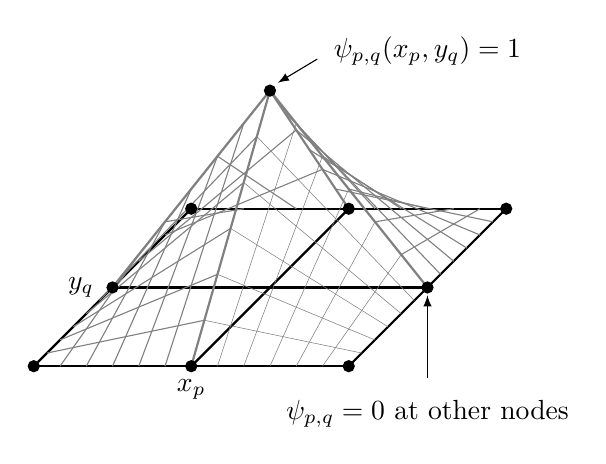
\begin{tikzpicture}[scale=0.5]

  % strong grid around elements
  \draw[thick] (0,0) -- (8,0);
  \draw[thick] (2,2) -- (10,2);
  \draw[thick] (4,4) -- (12,4);
  \draw[thick] (0,0) -- (4,4);
  \draw[thick] (4,0) -- (8,4);
  \draw[thick] (8,0) -- (12,4);

  \def\ytop{7};

  % tent lines
  \draw[gray,thick] (6,\ytop) -- (4,0);
  \draw[gray,thick] (6,\ytop) -- (2,2);
  \draw[gray,thick] (6,\ytop) -- (10,2);
  \draw[gray,thick] (6,\ytop) -- (8,4);

  \def\dx{(10.0-6.0)/6};
  \def\dy{(2.0-\ytop)/6};
  \foreach \jj in {1,...,5}
  {
       \draw[gray,very thin] ({6+\jj*\dx},{\ytop+\jj*\dy}) -- ({4+(4/6)*\jj},0.0);
  }

  \def\dx{(4.0-6.0)/6};
  \def\dy{(0.0-\ytop)/6};
  \foreach \jj in {1,...,5}
  {
       \draw[gray,very thin] ({6+\jj*\dx},{\ytop+\jj*\dy}) -- ({10-(2/6)*\jj},{2-(2/6)*\jj});
  }

  \def\dx{(2.0-6.0)/6};
  \def\dy{(2.0-\ytop)/6};
  \foreach \jj in {1,...,5}
  {
       \draw[gray,thin] ({6+\jj*\dx},{\ytop+\jj*\dy}) -- ({4-(4/6)*\jj},0.0);
  }

  \def\dx{(4.0-6.0)/6};
  \def\dy{(0.0-\ytop)/6};
  \foreach \jj in {1,...,5}
  {
       \draw[gray,thin] ({6+\jj*\dx},{\ytop+\jj*\dy}) -- ({2-(2/6)*\jj},{2-(2/6)*\jj});
  }

  \def\dx{(10.0-6.0)/6};
  \def\dy{(2.0-\ytop)/6};
  \foreach \jj in {1,...,5}
  {
       \draw[gray,thin] ({6+\jj*\dx},{\ytop+\jj*\dy}) -- ({8+(4/6)*\jj},4.0);
  }

  \def\dx{(8.0-6.0)/6};
  \def\dy{(4.0-\ytop)/6};
  \foreach \jj in {1,...,5}
  {
       \draw[gray,thin] ({6+\jj*\dx},{\ytop+\jj*\dy}) -- ({10+(2/6)*\jj},{2+(2/6)*\jj});
  }

  \def\dx{(2.0-6.0)/3};
  \def\dy{(2.0-\ytop)/3};
  \foreach \jj in {1,...,2}  % reduce clutter
  {
       \draw[gray,thin] ({6+\jj*\dx},{\ytop+\jj*\dy}) -- ({8-(4/3)*\jj},4.0);
  }

  \def\dx{(8.0-6.0)/3};
  \def\dy{(4.0-\ytop)/3};
  \foreach \jj in {1,...,2}
  {
       \draw[gray,thin] ({6+\jj*\dx},{\ytop+\jj*\dy}) -- ({2+(2/3)*\jj},{2+(2/3)*\jj});
  }

  % nodes in base plane
  \filldraw (0,0) circle (4pt);
  \filldraw (4,0) circle (4pt);
  \filldraw (8,0) circle (4pt);
  \filldraw (2,2) circle (4pt);
  %\filldraw (6,2) circle (4pt);   % (x_j,y_k) is at (6,2)
  \filldraw (10,2) circle (4pt);
  \filldraw (4,4) circle (4pt);
  \filldraw (8,4) circle (4pt);
  \filldraw (12,4) circle (4pt);

  % node at tent top
  \filldraw (6,\ytop) circle (4pt);

  % annotate
  \draw (10,\ytop+1.0) node {$\psi_{p,q}(x_p,y_q)=1$};
  \draw[-latex] (7.2,\ytop+0.8) -- (6.2,\ytop+0.2);
  \draw (10,-1.2) node {$\psi_{p,q}=0$ at other nodes};
  \draw[-latex] (10,-0.3) -- (10,1.8);

  % label center point
  \draw (4,-0.6) node {$x_p$};
  \draw (1.2,2) node {$y_q$};

\end{tikzpicture}

\caption{A hat function $\psi_{p,q} \in S^h$.}
\label{fig:of:q1hat}
\end{marginfigure}

When restricted to a particular element $\square_{ij}$, and then pulled-back to the reference element $\square_\ast$, the hat function $\psi_{p,q}$ is either identically zero or it is equal to one of the basis functions $\chi_\ell$.  That is, if corner $(\xi_\ell,\eta_\ell) \in \square_\ast$ corresponds to node $(x_p,y_q) \in \overline\Omega$, under the element map onto $\square_{ij}$, then
\begin{equation}
  \psi_{p,q}(x(\xi,\eta),y(\xi,\eta)) = \chi_\ell(\xi,\eta).  \label{eq:of:psionref}
\end{equation}
However, to evaluate $I[u]$ in \eqref{eq:of:sumoverelements} we will also want to compute gradients in the original $(x,y)$ variables:
\begin{equation}
  (\grad_{x,y} \psi_{p,q})(x(\xi,\eta),y(\xi,\eta)) = \left<\frac{2}{h_x}\frac{\partial\chi_\ell}{\partial \xi},\frac{2}{h_y}\frac{\partial\chi_\ell}{\partial \eta}\right>.   \label{eq:of:gradpsionref}
\end{equation}
Derivatives $\partial\chi_\ell/\partial \xi$ and $\partial\chi_\ell/\partial \eta$ can be found from formula \eqref{eq:of:chidefn} above.  Checking equation \eqref{eq:of:gradpsionref} is an easy exercise.

Suppose we have $v \in S_0^h$.  It can be represented using hat functions at the $N$ interior nodes
\begin{equation}
v(x,y) = \sum_{i=0}^{m_x-1} \sum_{j=0}^{m_y-1} v_{i,j} \psi_{i,j}(x,y) \label{eq:of:bilinearrepresentation}
\end{equation}
on $\Omega$.

On the other hand, suppose we have $v \in S^h$ with other boundary values.  It can be written almost the same as \eqref{eq:of:bilinearrepresentation} but with expanded summation ranges of $i=-1,0,\dots,m_x$ and $j=-1,0,\dots,m_y$, respectively, including the hat functions along the boundary.  We will see that \PETSc makes it easy to represent any function in $S^h$ through ``ghost values'' off the edge of our grid of interior nodes.

A bilinear function on element $\square_{i,j}$ pulls-back to the reference element $\square_\ast$, using local node numbering, as
\begin{equation}
v(\xi,\eta) = \sum_{\ell=0}^3 v_\ell \chi_\ell(\xi,\eta)  \qquad \text{on } \,\square_\ast. \label{eq:of:bilinearref}
\end{equation}
The coefficient $v_\ell$ is equal to $v_{r,s} = v(x_r,y_s)$ for $(x_r,y_s)\in\square_{i,j}$ corresponding under the element map to $(\xi_\ell,\eta_\ell) \in \square_\ast$.  Also, by \eqref{eq:of:gradpsionref} the $(x,y)$ gradient has formula:
\begin{equation}
  (\grad_{x,y} v)(\xi,\eta) = \left<\frac{2}{h_x} \sum_{\ell=0}^3 v_\ell \frac{\partial\chi_\ell}{\partial \xi}, \frac{2}{h_y} \sum_{\ell=0}^3 v_\ell \frac{\partial\chi_\ell}{\partial \eta}\right>. \label{eq:of:gradrepref}
\end{equation}


\section{Quadrature}

We do not plan to exactly-compute the integrals in \eqref{eq:of:sumoverelements}.  For general $p$ it would be quite challenging to exactly-integrate the term ``$|\grad u|^p$.''  Instead we will use numerical integration, also known a \emph{quadrature}.

First, change-of-variables transfers the integral to the reference element: If $v(x,y)$ is any integrable function on element $\square_{i,j}$ then, using the element map and \eqref{eq:of:elementjacobian}, we have
\begin{equation}
\int_{\square_{ij}} v(x,y)\,dx\,dy = \frac{h_x h_y}{4} \int_{\square_\ast} v(\xi,\eta) \,d\xi\,d\eta \label{eq:of:changeofvars}
\end{equation}
where $v(\xi,\eta)=v(x(\xi,\eta),y(\xi,\eta))$.

Next, recall Gauss-Legendre quadrature on integrals in one dimension \citep{GreenbaumChartier2012}:
\begin{equation}
\int_{-1}^1 f(z)\,dz \approx \sum_{q=0}^{n-1} w_q f(z_q).  \label{eq:of:gauss}
\end{equation}
For degrees $n=1,2,3$, the quadrature \emph{nodes} $z_q$ and \emph{weights} $w_q$ for integration over the interval $[-1,1]$ are given in Table \ref{tab:of:gauss}.  The degree $n$ rule is exact for polynomials of degree $2n-1$ and less.

\begin{table}[h]
\vspace{0.1in}

\begin{tabular}{lll}
$n$\phantom{foobar} & nodes $z_q$\phantom{foo} & weights $w_q$ \\ \hline
$1$ & $0$ & $2$ \\
$2$ & $-\frac{1}{\sqrt{3}}, +\frac{1}{\sqrt{3}}$ & $1,1$ \\
$3$ & $-\sqrt{\frac{3}{5}}, 0, +\sqrt{\frac{3}{5}}$ & $\frac{5}{9}, \frac{8}{9}, \frac{5}{9}$ \\
\end{tabular}

\vspace{0.1in}
\caption{Nodes and weights for low-degree Gauss-Legendre quadrature rules, for integrals \eqref{eq:of:gauss}.} \label{tab:of:gauss}
\end{table}

Rule \eqref{eq:of:gauss} extends to a product formula for integrals over $\square_\ast$:
\begin{equation}
\int_{\square_\ast} v(\xi,\eta) \,d\xi\,d\eta \approx \sum_{r=0}^{n-1} \sum_{s=0}^{n-1} w_r w_s v(z_r,z_s).  \label{eq:of:tensorgauss}
\end{equation}
The $n=2,3$ cases are shown in Figure \ref{fig:of:gausstwod}, while the $n=1$ rule is simply the midpoint rule on $\square_\ast$.

Formulas \eqref{eq:of:bilinearref}, \eqref{eq:of:gradrepref}, \eqref{eq:of:changeofvars}, and \eqref{eq:of:tensorgauss} combine to give an easily-computed approximation of integral in \eqref{eq:of:sumoverelements}.  On the reference element we define
\begin{equation}
G_{ij}(\xi,\eta) = \left[\frac{1}{p} |\grad u|^p - fu\right]_{\square_\ast} \label{eq:of:integrandheuristic}
\end{equation}
using the nodal values of $u$ and $f$ on element $\square_{ij}$.  (The details are in Exercise \ref{chap:of}.\ref{exer:of:integrand}.)  Then formula \eqref{eq:of:sumoverelements} becomes
\begin{equation}
I^h[u] = \frac{h_x h_y}{4} \quad \underbrace{\sum_{i=0}^{m_x} \sum_{j=0}^{m_y}}_{\begin{smallmatrix} \text{sum} \\ \text{over} \\ \text{elements} \end{smallmatrix}} \quad \underbrace{\sum_{r=0}^{n-1} \sum_{s=0}^{n-1}}_{\begin{smallmatrix} \text{sum} \\ \text{over} \\ \text{quadrature points} \end{smallmatrix}} \, w_r w_s G_{ij}(z_r,z_s) \label{eq:of:quadraturesumoverelements}
\end{equation}
We now have enough detail for a prototype implementation.

\newcommand{\gausssanspts}{
  % (xi,eta) reference element is square with half-width 1
  \draw[->,very thin] (-1.2,0.0) -- (1.2,0.0) node[below] {\small $\xi$};
  \draw[->,very thin] (0.0,-1.2) -- (0.0,1.2) node[left] {\small $\eta$};
  \draw[line width=1.5pt] (1.0,1.0) -- (-1.0,1.0) -- (-1.0,-1.0) -- (1.0,-1.0) -- cycle;
}

\begin{figure}
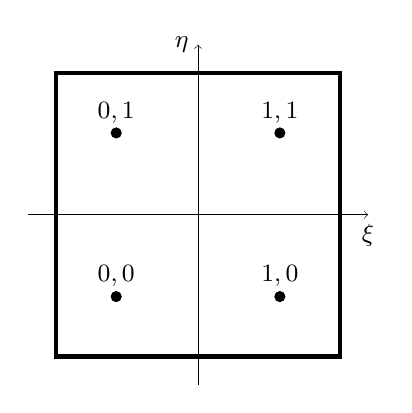
\begin{tikzpicture}[scale=1.8]
\gausssanspts
\pgfmathsetmacro\gl{1.0/sqrt(3.0)}
\foreach \x [count=\RR from 0] in {-\gl,\gl} {
    \foreach \y [count=\SS from 0] in {-\gl,\gl} {
         \filldraw (\x,\y) circle (1.0pt) node[above] {\small $\RR,\SS$};
    }
}
\end{tikzpicture}
\qquad\qquad
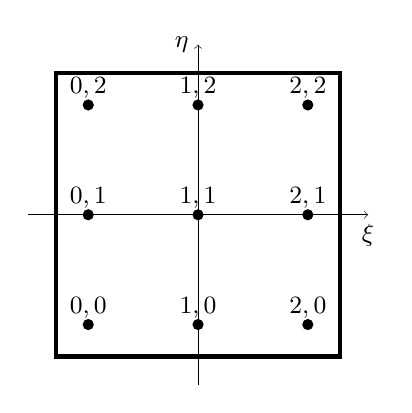
\begin{tikzpicture}[scale=1.8]
\gausssanspts
\pgfmathsetmacro\gl{sqrt(3.0/5.0)}
\foreach \x [count=\RR from 0] in {-\gl,0,\gl} {
    \foreach \y [count=\SS from 0] in {-\gl,0,\gl} {
         \filldraw (\x,\y) circle (1.0pt) node[above,yshift=-0.4mm] {\small $\RR,\SS$};
    }
}
\end{tikzpicture}
\caption{The $n=2$ (left) and $n=3$ (right) Gauss-Legendre quadrature points on the reference element $\square_\ast$.  Points $(z_r,z_s)$ are labeled as ``$r,s$''.  See equation \eqref{eq:of:tensorgauss} and Table \ref{tab:of:gauss}.}
\label{fig:of:gausstwod}
\end{figure}


\section{Objective-only implementation}

Our program \texttt{plap.c} is displayed in eight parts, Codes \ref{code:plapCtx}--\ref{code:plapFun}.  However, Code \ref{code:plapFun}, which implements the weak form \eqref{eq:of:plapweakform}, is shown after we get it running initially using only an implementation of objective functional \eqref{eq:of:functional}, that is, sum \eqref{eq:of:quadraturesumoverelements}.

Code \ref{code:plapCtx} declares a ``context'' \texttt{struct PLapCtx} which will be needed in the call-back functions \texttt{FormObjectiveLocal()} (Code \ref{code:plapObj}) and \texttt{FormFunctionLocal()} (Code \ref{code:plapFun}).  Defaults and \PETSc options are then set in the \texttt{ConfigureCtx()} function.  Note that exponent $p$ defaults to 4.

\cinputpart{plap.c}{\CODELOC}{Declare and configure a context.}{I}{//STARTCTX}{//ENDCTX}{code:plapCtx}

Next, in Code \ref{code:plapBI} we declare a function \texttt{BoundaryG()} for computing the boundary values $g(x,y)$.  (In fact this is just the exact solution $u(x,y)$ from \eqref{eq:of:exactsolution}.)  The function \texttt{SetGLocal()} sets boundary conditions at the ghosted points of the \texttt{Local} \pVec which stores $g$.  Also the function \texttt{InitialIterate()} sets the initial values of $u$ for the Newton iteration, by linearly-interpolating the boundary values into the interior nodes.

The third part, Code \ref{code:plapEx}, implements exact solution \eqref{eq:of:exactsolution} and computes the corresponding source term $f$ from PDE \eqref{eq:of:plapstrongform}.  In this case $f$ is computed at all grid points, including the ghost points of the \texttt{Local} \pVec which holds $f$, while the exact values of $u$ are only computed at the interior points; \texttt{uexact} is a \texttt{Global} \pVec.\sidenote{For ``fairness'' we will store the exact values of $u$ in a \pVec \texttt{uexact} which is unavailable to the call-back functions used in solving the PDE.}

A main concern in Codes \ref{code:plapBI} and \ref{code:plapEx} is that we will be able to integrate $u$, its derivatives, and $f$ on each element.  This requires ghosted values of $f$ and $g$.  These ghosted values are used in Codes \ref{code:plapTool}, \ref{code:plapObj}, and \ref{code:plapFun} below.

We show FEM tools in Code \ref{code:plapFEM}.  These are generic to any $Q^1$ method in 2D which is based on a reference element.  We evaluate basis functions $\chi_\ell$, and their partial derivatives, at points $(\xi,\eta) \in \square_\ast$.  We also implement formulas \eqref{eq:of:chidefn}, \eqref{eq:of:bilinearref}, and \eqref{eq:of:gradrepref}.  Note that a two-element \texttt{struct gradRef} holds the components of a gradient at a point.  We also declare nodes and weights for degree $n=1,2,3$ Gauss-Legendre quadrature, with values from Table \ref{tab:of:gauss}.

\cinputpart{plap.c}{\CODELOC}{Set boundary values and initial iterate.  The boundary values set the ghosted nodes of a \texttt{Local} \pVec.}{II}{//STARTBDRYINIT}{//ENDBDRYINIT}{code:plapBI}

Next, Code \ref{code:plapTool} has functions of convenience; these allow us to avoid code duplication in \texttt{FormObjectiveLocal()} and \texttt{FormFunctionLocal()}.  First is a function \texttt{GetUorG()} which evaluates either $u(x,y)$ or $g(x,y)$ according to whether a point $(x_i,y_j)\in\overline\Omega$ is an interior or boundary node.  Then there are methods which compute point-wise inner products $\grad u\cdot \grad v$ and powers $|\grad u|^P$ from nodal values.

\cinputpart{plap.c}{\CODELOC}{Compute exact solution $u(x,y)$ from \eqref{eq:of:exactsolution}, and the corresponding source function $f(x,y)$.}{III}{//STARTEXACT}{//ENDEXACT}{code:plapEx}


In Code \ref{code:plapObj} we compute the discrete objective functional $I^h[u]$, from \eqref{eq:of:quadraturesumoverelements}, in parallel.  The basic structure is that each rank computes its portion of the sum over all elements.  A local total \texttt{lobj} is incremented in the loop over owned elements by the line
\begin{code}
    lobj += wq[n-1][r] * wq[n-1][s] * ObjIntegrand(info,f,u,zq[n-1][r],zq[n-1][s],user->p);
\end{code}
which uses both the quadrature weights $w_q$ and nodes $z_q$ (Code \ref{code:plapFEM}).  Function \texttt{ObjIntegrand()} implements $G_{ij}(\xi,\eta)$ from \eqref{eq:of:integrandheuristic}.  Once the local contribution is fully-summed, a reduction across the MPI communicator puts the value of $I^h[u]$ into variable \texttt{obj} on each rank:
\begin{code}
    MPI_Allreduce(&lobj,obj,1,MPIU_REAL,MPIU_SUM,com);
\end{code}

\cinputpart{plap.c}{\CODELOC}{Tools for any 2D $Q^1$ FEM method.}{IV}{//STARTFEM}{//ENDFEM}{code:plapFEM}

However, implementing the objective function requires us to be clearer than we have been so far on the parallel distribution of nodes and elements.  To do a sum over elements we must assign unique ownership of an element to a rank (process).

\cinputpart{plap.c}{\CODELOC}{Functions needed for evaluation of boundary values and functions of the gradient $\grad u$.}{V}{//STARTTOOLS}{//ENDTOOLS}{code:plapTool}

Figure \ref{fig:of:parallelgrid} shows the scheme we have implemented.  The interior nodes are distributed across the processes in the obvious way.  That is, \PETSc's \pDMDA object treats the grid of interior nodes here just as it did the grid of all nodes in Chapter \ref{chap:st}.  Regarding the elements, we decide that each rank owns those which are down and left from an owned node.  However, we also decide that ranks which own $i=m_x-1$ or $j=m_y-1$ nodes, that is, ranks which own the upper or right edges of the grid, also own the elements above and to the right of these nodes.

\newcommand{\gridsansowners}{
  % grid
  \draw[line width=1.0pt] (0.0,0.0) -- (0.0,1.0) -- (1.0,1.0) -- (1.0,0.0) -- cycle;
  \pgfmathsetmacro\fifth{1.0/5.0}
  \draw[xstep=\fifth,ystep=\fifth,black,thin] (0.0,0.0) grid (1.0,1.0);
  % prominent nodes
  \foreach \x in {1,...,4} {
    \foreach \y in {1,...,4} {
        \filldraw (\x * \fifth,\y * \fifth) circle (0.4pt);
    }
  }
  % tick marks for i
  \draw[line width=1.0pt] (0.2,-0.04) -- (0.2,0.02);
  \draw[line width=1.0pt] (0.8,-0.04) -- (0.8,0.02);
  \node[yshift=-4mm] at (0.2,0.0) {\small $i=0$};
  \node[yshift=-4mm] at (0.8,0.0) {\small $m_x\!-\!1$};
  % tick marks for j
  \draw[line width=1.0pt] (-0.04,0.2) -- (0.02,0.2);
  \draw[line width=1.0pt] (-0.04,0.8) -- (0.02,0.8);
  \node[xshift=-6mm] at (0.0,0.2) {\small $j=0$};
  \node[xshift=-6.5mm] at (0.0,0.8) {\small $m_y\!-\!1$};
}

\begin{figure}
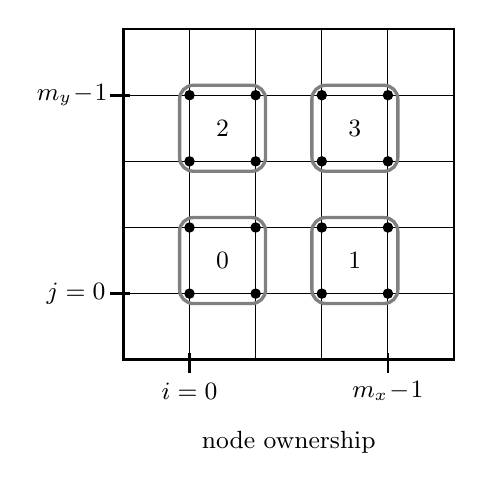
\begin{tikzpicture}[scale=4.2]
\gridsansowners
\pgfmathsetmacro\half{0.5*\fifth}
\pgfmathsetmacro\AA{0.15*\fifth}
\foreach \x in {1,3} {
    \foreach \y in {1,3} {
        \draw[very thick,rounded corners=5pt,gray] (\x*\fifth-\AA,\y*\fifth-\AA) -- (\x*\fifth+\fifth+\AA,\y*\fifth-\AA) -- (\x*\fifth+\fifth+\AA,\y*\fifth+\fifth+\AA) -- (\x*\fifth-\AA,\y*\fifth+\fifth+\AA) -- cycle;
    }
}
\node at (\fifth+\half,\fifth+\half) {\small $0$};
\node at (3*\fifth+\half,\fifth+\half) {\small $1$};
\node at (\fifth+\half,3*\fifth+\half) {\small $2$};
\node at (3*\fifth+\half,3*\fifth+\half) {\small $3$};
\node at (0.5,-0.25) {\small node ownership};
\end{tikzpicture}
\quad
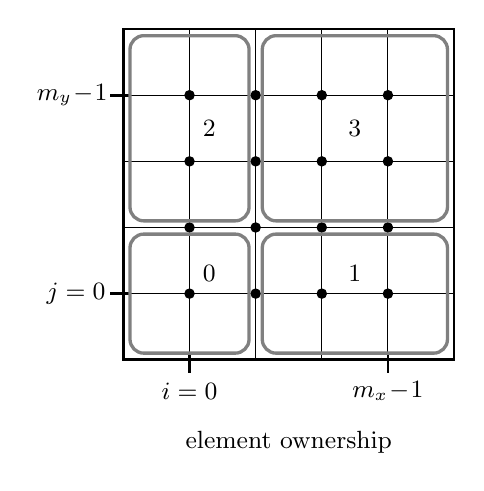
\begin{tikzpicture}[scale=4.2]
\gridsansowners
\pgfmathsetmacro\half{0.5*\fifth}
\pgfmathsetmacro\bit{0.3*\fifth}
\pgfmathsetmacro\BB{0.1*\fifth}
\draw[very thick,rounded corners=5pt,gray] (\BB,\BB) -- (2*\fifth-\BB,\BB) -- (2*\fifth-\BB,2*\fifth-\BB) -- (\BB,2*\fifth-\BB) -- cycle;
\draw[very thick,rounded corners=5pt,gray] (2*\fifth+\BB,\BB) -- (5*\fifth-\BB,\BB) -- (5*\fifth-\BB,2*\fifth-\BB) -- (2*\fifth+\BB,2*\fifth-\BB) -- cycle;
\draw[very thick,rounded corners=5pt,gray] (\BB,2*\fifth+\BB) -- (2*\fifth-\BB,2*\fifth+\BB) -- (2*\fifth-\BB,5*\fifth-\BB) -- (\BB,5*\fifth-\BB) -- cycle;
\draw[very thick,rounded corners=5pt,gray] (2*\fifth+\BB,2*\fifth+\BB) -- (5*\fifth-\BB,2*\fifth+\BB) -- (5*\fifth-\BB,5*\fifth-\BB) -- (2*\fifth+\BB,5*\fifth-\BB) -- cycle;
\node at (\fifth+\bit,\fifth+\bit) {\small $0$};
\node at (3*\fifth+\half,\fifth+\bit) {\small $1$};
\node at (\fifth+\bit,3*\fifth+\half) {\small $2$};
\node at (3*\fifth+\half,3*\fifth+\half) {\small $3$};
\node at (0.5,-0.25) {\small element ownership};
\end{tikzpicture}
\medskip

\caption{Parallel distribution of interior nodes (left) and elements (right) in a $m_x=4$, $m_y=4$ grid.  Here there are four processes with ranks $0,1,2,3$.}
\label{fig:of:parallelgrid}
\end{figure}

\cinputpart{plap.c}{\CODELOC}{Implement \eqref{eq:of:quadraturesumoverelements} for the objective function $I^h[u]$.}{VI}{//STARTOBJECTIVE}{//ENDOBJECTIVE}{code:plapObj}

Our scheme implies a slight load imbalance in the sense that ranks along the upper and right-hand side of the grid do more work.  This imbalance is quite tolerable if each rank owns a significant block of nodes, e.g.~a squarish block of thousands of interior nodes.

\cinputpart{plap.c}{\CODELOC}{In \texttt{main()} we set up \pDMDA, some \pVecs, and the \pSNES.  Then we solve and compute the error.}{VII}{//STARTMAIN}{//ENDMAIN}{code:plapMain}

The main part, Code \ref{code:plapMain}, calls the various functions in the previous parts, of course.  We set up \pDMDA, some \pVecs, and \pSNES objects.  Note that we use \texttt{DMCreateGlobalVector()} on \texttt{u} and \texttt{uexact}, but \texttt{DMCreateLocalVector()} on the \pVecs which hold $f$ and $g$.  The latter \pVecs do not change during the run, so we never need to call \texttt{DMGlobalToLocalBegin/End()}.  Also, we tell the \pDMDA to use objective function \texttt{FormObjectiveLocal()} by calling \texttt{DMDASNESSetObjectiveLocal()}.  Similarly, we call \texttt{DMDASNESSetFunctionLocal()} to tell the \pDMDA about \texttt{FormFunctionLocal()}; see Code \ref{code:plapFun} for the implementation.

Then we call \texttt{SNESSolve()}, compute the error, and destroy all the objects at the end.  Regarding that last \texttt{Destroy()} step, the reader might start running the program by confirming that it has no memory leaks:
\begin{cline}
$ cd c/ch5/
$ make plap
...
$ valgrind ./plap
...
\end{cline}
%$

The parts above show the objective-only implementation.  To use it requires option \texttt{-snes\_fd\_function}, which does finite differencing on the objective functional $I^h[u]$, equation \eqref{eq:of:quadraturesumoverelements}, to get its gradient $\grad I^h[u]$.  Then the \pSNES solves $F(u) = \grad I^h[u] = 0$.

Of course, even with a residual function $F(u)$ we still need a Jacobian for Newton's method.  To get this we ask \PETSc to finite difference \emph{again}, using either \texttt{-snes\_fd} or \texttt{-snes\_mf}.  Recall from Chapter \ref{chap:nl} that we can ask \PETSc to count C function evaluations, to confirm that only the objective function is evaluated:
\begin{cline}
$ ./plap -snes_fd_function -snes_fd -log_summary | grep Eval
SNESObjectiveEval    2198 1.0 1.8496e-01 1.0 ...
SNESJacobianEval       7 1.0 2.1275e-01 1.0 ...
\end{cline}
%$
On the default ($3\times 3$ interior nodes) grid we have evaluated the objective functional 2198 times, already a warning about the scalability of this method.\sidenote{The Jacobian evaluation counts report calls to \PETSc's finite difference Jacobian method.}

Actually, experience from Chapter \ref{chap:nl} suggests using a ``coloring'' method, available for our \pDMDA-managed structured grid.  This reduces the evaluation count, especially on a once-refined $5 \times 5$ grid:
\begin{cline}
$ ./plap -snes_fd_function -snes_fd -da_refine 1 -log_summary | grep ObjectiveEval
SNESObjectiveEval   20539 1.0 1.5497e+00 1.0 ...
$ ./plap -snes_fd_function -snes_fd_color -da_refine 1 -log_summary | grep ObjectiveEval
SNESObjectiveEval    5410 1.0 4.8340e-01 1.0 ...
\end{cline}
These remain disturbingly-large evaluation counts.

Given that we have an implementation with an exact solution, we want to see convergence:\sidenote{Recall the \texttt{alias} set in Chapter \ref{chap:ls}: \texttt{timer='time -f "real \%e"'}.}
\begin{cline}
$ for LEV in 0 1 2 3; do
> timer ./plap -snes_fd_color -snes_fd_function -snes_converged_reason -da_refine $LEV
> done
grid of 3 x 3 = 9 interior nodes (16 elements)
Nonlinear solve converged due to CONVERGED_FNORM_ABS iterations 6
numerical error:  |u-u_exact|/|u_exact| = 0.0080805
real 0.22
grid of 5 x 5 = 25 interior nodes (36 elements)
Nonlinear solve converged due to CONVERGED_FNORM_ABS iterations 7
numerical error:  |u-u_exact|/|u_exact| = 0.00292891
real 0.50
grid of 9 x 9 = 81 interior nodes (100 elements)
Nonlinear solve did not converge due to DIVERGED_LINEAR_SOLVE iterations 8
numerical error:  |u-u_exact|/|u_exact| = 0.000925284
real 2.73
grid of 17 x 17 = 289 interior nodes (324 elements)
Nonlinear solve did not converge due to DIVERGED_LINE_SEARCH iterations 20
numerical error:  |u-u_exact|/|u_exact| = 0.00025817
real 47.74
\end{cline}
%$
This is evidence of convergence indeed, with reductions of the error by factors close to $O(\Delta x^2)$, but the rest of the evidence provides copious warnings.  First, performance is terrible, presumably coming from excessive objective evaluation.  Secondly, though errors are small, suggesting that convergence occurred, on the two finer grids we get divergence.  Such troubles are no surprise, as the Jacobian is computed by finite differencing a gradient computed by finite differences!\sidenote{Thank goodness we have 64 bit \texttt{double} precision, to get even this far.}

However, we can see from the small errors that the FEM of this Chapter has allowed us to numerically-solve the $p$-Laplacian PDE using \PETSc's ability to minimize a function.  This is a useful capability for prototyping, and for providing a redundant capability for checking the correctness of better approaches.  Let us move on to one of those, namely actually implementing the weak form \eqref{eq:of:plapweakform}, which is the missing gradient.


\section{Residual function (gradient) implementation}

As we will see, there are significant limitations to the objective-only implementation above.  Grids other than the very coarsest lead to unreasonable numbers of evaluations of the objective function.  Furthermore the quality of the numerically-approximated finite difference gradient of the objective function, that is, of the residual function, is low.  So we take the next step in user-written code, by implementing a residual function.

Recall \eqref{eq:of:plapweakform}, the weak form of the $p$-Laplacian equation, which says $\grad I[u](v) = 0$ for all $v\in W_0^{1,p}(\Omega)$.  The corresponding statement for $u\in S_g^h$ and all $v \in S_0^h$ can be written out in the basis of hat functions.

Thus we require $u$ to satisfy \eqref{eq:of:plapweakform} for $v=\psi_{ij}$ at each of the $N$ interior nodes:
\begin{equation}
\int_\Omega |\grad u|^{p-2} \grad u \cdot \grad \psi_{ij} - f \psi_{ij} = 0. \label{eq:of:weakformbasis}
\end{equation}
Note that the support of $\psi_{ij}$ is localized around the node $(x_i,y_j)$,
    $$\operatorname{supp} \psi_{ij} = \square_{ij} \cup \square_{i+1,j} \cup \square_{i,j+1} \cup \square_{i+1,j+1},$$
so in fact the integral in \eqref{eq:of:weakformbasis} is over these four elements.  Also, on the reference element we define
\begin{equation}
H_{ijcd}(\xi,\eta) = \left[|\grad u|^{p-2} \grad u \cdot \grad \chi_{[ij]} - f \chi_{[ij]}\right]_{\square_\ast} \label{eq:of:weakformintegrandref}
\end{equation}
where $\chi_{[ij]}$ denotes the basis function $\chi_\ell$ corresponding to $\psi_{ij}$--- recall equation \eqref{eq:of:psionref}---and where we use the nodal values of $u$ and $f$ on element $\square_{i+c,j+d}$ for $c,d=0,1$.  (Compare equation \eqref{eq:of:integrandheuristic}.  The details for equation \eqref{eq:of:weakformintegrandref} are in Exercise \ref{chap:of}.\ref{exer:of:weakformintegrand}.)  Finally, we do the element integrals implied by \eqref{eq:of:weakformbasis} by using quadrature \eqref{eq:of:tensorgauss}.

In these terms, we rewrite \eqref{eq:of:weakformbasis} as this equation,
\begin{equation}
0 = \frac{h_x h_y}{4} \sum_{c=0}^1 \sum_{d=0}^1 \sum_{r=0}^{n-1} \sum_{s=0}^{n-1} w_r w_s H_{ijcd}(z_r,z_s).  \label{eq:of:weakformdetail}
\end{equation}
There is one such nonlinear equation for each of the $N$ interior nodes $(x_i,y_j)$.  Solving this system of equations is intended to determine all $N$ values $u_{ij}$.

\cinputpart{plap.c}{\CODELOC}{FIXME}{VIII}{//STARTFUNCTION}{//ENDFUNCTION}{code:plapFun}


\section{FIXME looking at result and performance}

% Do you want the solution of the linear system before the line search (line search may shrink the vector) use -ksp_view_solution or the actual update selected by Newton -snes_monitor_solution_update
%   If you use the master branch of PETSc then both of these flags take the option
%    [ascii or binary or draw][:filename][:viewer format]
%  allowing printing as ascii, binary or drawing the solution in a window (Drawing only works for DMDA 1d or 2d).
%   Barry

FIXME 

% -log_summary | grep Eval


\section{Exercises}

\renewcommand{\labelenumi}{\arabic{chapter}.\arabic{enumi}\quad}
\renewcommand{\labelenumii}{(\alph{enumii})}
\begin{enumerate}
\item  \label{exer:of:twoproperties}  \emph{This two-part exercise is a mathematical excursion which some readers may wish to skip.}
  \begin{enumerate}
  \item For $1 \le p < \infty$, prove coercivity \eqref{eq:of:coercivity} of functional $I[u]$, defined in \eqref{eq:of:functional}, on $W_0^{1,p}(\Omega)$.  (\emph{Hints}:  Use Poincar\`e inequality \citep[Theorem 6.30]{AdamsFournier2003} to convert to replace the leading term with the full $W^{1,p}$ norm.  Use Young's inequality with $\epsilon>0$ \citep[Appendix B]{Evans2010} for the ``$-fu$'' term.  Now choose $\eps$ appropriately.)
  \item For $1 < p < \infty$, prove strict convexity \eqref{eq:of:convexity} of functional $I[u]$ on $W_0^{1,p}(\Omega)$.  (\emph{Hint}:  The argument in section 5.3 of \citet{Ciarlet2002} suffices.)
  \end{enumerate}
 
\item \label{exer:of:checkexactformulas} For the exact solution \eqref{eq:of:exactsolution}, define $C = |\grad u|^{p-2}$ and $D^2=(x+1)^2 + (y+1)^2$ and show that
    $$C = \left[(x+1)^2 (y+1)^2 D^2\right]^{(p-2)/2}$$
and that $\grad C = (p-2) C \left<\gamma_1,\gamma_2\right>$ where
    $$\gamma_1 = \frac{1}{x+1}+ \frac{x+1}{D^2}, \quad \gamma_2 = \frac{1}{y+1}+ \frac{y+1}{D^2}.$$
Also show that $\Div \grad u = D^2$.  Thus strong form \eqref{eq:of:plapstrongform} implies an implementable formula for the source function,
    $$f = - \Div \left(C \grad u\right) = - \grad C \cdot \grad u - C\, \Div \grad u.$$
Note that \texttt{ExactRHSLocal()} in \texttt{plap.c} implements these formulas.

\item \label{exer:of:checkexactbounds} For the exact solution \eqref{eq:of:exactsolution}, show \eqref{eq:of:coeffbounds}.

\item Show that $S^h$ is a linear subspace of $W^{1,p}(\Omega)$ with dimension $(m_x+2)(m_y+2)$, and that $S_0^h$ has dimension $m_x m_y$.  What precisely is meant by saying $g$ is ``(appropriately) piece-wise linear on $\partial\Omega$'' in the definition of $S_g^h$ on page \pageref{eq:of:Sghdefn}?  Is our use of exact solution \eqref{eq:of:exactsolution} to give $g$ ``appropriate'' in this sense?

\item  Use \eqref{eq:of:refcorners} and \eqref{eq:of:chidefn} to show that the two forms of the reference map \eqref{eq:of:referencemap} are the same.  Then use \eqref{eq:of:chidefn}, \eqref{eq:of:referencemap}, and \eqref{eq:of:psionref} to derive \eqref{eq:of:gradpsionref}.

\item By testing against the integral
    $$\int_{\square_\ast} (1+\xi)^k + (1+\eta)^k\,d\xi\, d\eta = \frac{2^{k+3}}{k+1}$$
for $k=0,1,\dots,6$, confirm that the $n=1,2,3$ Gauss-Legendre quadrature formulas listed in the text will exactly integrate degree $2n-1$ degree polynomials, but not degree $2n$ polynomials, on the reference element.  (\emph{Use the computer language of your choice.})
% solution:  matlab/testgauss2d.m

\item \label{exer:of:integrand}  Show that \eqref{eq:of:integrandheuristic} is, in detail,
\begin{align*}
G_{ij}(\xi,\eta) &= \frac{1}{p} \left[\frac{4}{h_x^2} \left(\sum_{\ell=0}^3 u_\ell \frac{\partial\chi_\ell}{\partial \xi}\right)^2 + \frac{4}{h_y^2} \left(\sum_{\ell=0}^3 u_\ell \frac{\partial\chi_\ell}{\partial \eta}\right)^2\right]^{p/2} \\
  &\qquad - \left(\sum_{\ell=0}^3 f_\ell \chi_\ell\right) \left(\sum_{\ell=0}^3 u_\ell \chi_\ell\right)
\end{align*}
where $u_\ell$ and $f_\ell$ are local-node-numbered values of $u$ and $f$ on element $\square_{ij}$.

\item \label{exer:of:weakformintegrand}  Show that \eqref{eq:of:weakformintegrandref} is, in detail,
\begin{align*}
H_{ijcd}(\xi,\eta) &= \left[\frac{4}{h_x^2} \left(\sum_{\ell=0}^3 u_\ell \frac{\partial\chi_\ell}{\partial \xi}\right)^2 + \frac{4}{h_y^2} \left(\sum_{\ell=0}^3 u_\ell \frac{\partial\chi_\ell}{\partial \eta}\right)^2\right]^{(p-2)/2} \\
  &\qquad \cdot \left[\frac{4}{h_x^2} \left(\sum_{\ell=0}^3 u_\ell \frac{\partial\chi_\ell}{\partial \xi}\right) \frac{\partial\chi_{[ij]}}{\partial \xi} + \frac{4}{h_y^2} \left(\sum_{\ell=0}^3 u_\ell \frac{\partial\chi_\ell}{\partial \eta}\right) \frac{\partial\chi_{[ij]}}{\partial \eta}\right] \\
  &\quad - \left(\sum_{\ell=0}^3 f_\ell \chi_\ell\right) \chi_{[ij]}
\end{align*}

\item Figure \ref{fig:of:cartoonfunctional} shows the graph of $\Phi(x,y)=\tfrac{1}{4}(x^4+y^4) - 2x + 2y$, a cartoon for the $p$-Laplacian functional $I[u]$ in the case $p=4$.  Solve
    $$\min_{x,y} \Phi(x,y)$$
by hand.  Now write a \PETSc code \texttt{cartoon.c} to solve this problem, starting with a code that only implements $\Phi(x,y)$ by a function \texttt{FormObjective()} and a call to \texttt{SNESSetObjective()}.  After checking that it works using ``\texttt{./cartoon -snes\_fd\_function -snes\_fd},'' add a function \texttt{FormFunction()} and a call to \texttt{SNESSetFunction()} and check that now ``\texttt{./cartoon -snes\_fd}'' works.  (\emph{Hint}:  \texttt{expcircle.c} from Chapter \ref{chap:nl} is a convenient starting point for your code.)
% solution:  c/ch5/solns/cartoon.c

\item Comment-out the parts of \texttt{plap.c} shown in Code \ref{code:plapFun}, including the \texttt{DMDASNESSetFunctionLocal()} line which tells the \pDMDA and \pSNES about the residual-evaluation function.  You now have a truly ``objective-only'' code.  Confirm that
\begin{cline}
./plap -snes_fd -snes_fd_function
\end{cline}
works, but that
\begin{cline}
./plap -snes_fd
./plap -snes_mf
\end{cline}
do not.  Confirm the evaluation-counting results in the text with ``\texttt{-log\_summary | grep Eval}''.
%FIXME:  what is "./plap -snes_fd_function" doing?


\item \label{exer:of:regularize}  The solution of the $p$-Laplacian equation shown in this Chapter is actually rather ``dangerous'' in the sense that the equation is solved as though it is uniformly elliptic.  Making that assumption is solution- and method-dependent; see \eqref{eq:of:coeffbounds}.  For this reason it is common to \emph{regularize} the $p$-Laplacian by inserting a constant $\eps>0$ so that the weak form \eqref{eq:of:plapweakform} becomes
\begin{equation}
\int_\Omega \left(|\grad u|^2+\eps^2\right)^{(p-2)/2} \grad u \cdot \grad v - f v = 0, \label{eq:of:plapweakformreg}
\end{equation}
and thus uniform ellipticity is guaranteed in a ball in $W^{1,p}(\Omega)$ around any solution.  Add this as an optional regularization in \texttt{plap.c}. Specifically, modify function \texttt{FormFunctionLocal()}, but note that \texttt{FormObjectiveLocal()} can remain unchanged.\sidenote{Following this advice means that \texttt{FormFunctionLocal()} only computes an approximate gradient of the objective functional.  However, the line search in the Newton iteration suffers very little as a consequence.}  Run the code with small nonzero values of $\eps$, and note the largest $\eps$ value which still gets 1\% agreement with unregularized results on a selection of grids.

\item \label{exer:of:regularizebad}  Continue the last exercise, but now change the manufactured solution \eqref{eq:of:exactsolution}, i.e.~the function \texttt{ExactRHSLocal()} in \texttt{plap.c}, to be
\begin{equation}
    u(x,y) = \frac{1}{2} x^2 y^2. \label{eq:of:exactsolutionbad}
\end{equation}
Now $\grad u \to 0$ as $(x,y)\to(0,0)$ in $\Omega$ so that $|\grad u|^{p-2}$ is not bounded-below by a positive constant; compare \eqref{eq:of:coeffbounds}.  Show that $\eps$-regularized cases can converge on fine grids but that the unregularized ($\eps=0$) method runs into trouble.

\item One may approximate the strong form PDE \eqref{eq:of:plapstrongform} by finite differences on a structured grid just like that used in Chapter \ref{chap:st}.  Do so, in a \pSNES-using code \texttt{plapfd.c} that implements the nonlinear residual and the same manufactured solution as here.  At least initially, skip the Jacobian implementation.  Use \texttt{-snes\_fd\_color} and compare to results in this chapter.  What are the differences in your code relative to the code \texttt{plap.c}?

\item It is common to linearize the strong form PDE \eqref{eq:of:plapstrongform} to get an iterative scheme
\begin{equation}
- \Div\left(|\grad u^{(k-1)}|^{p-2} \grad u^{(k)}\right) = f,
\label{eq:of:picard}
\end{equation}
a \emph{Picard} iteration.  Implement this method by adding a function \texttt{FormPicardLocal()} to \texttt{plap.c}.  This function computes and assembles a \pMat for the left side, so that \eqref{eq:of:picard} is a linear equation $A\bu = \bb$ at each iteration.  Use \texttt{MatSetValuesStencil()} to insert entries into the \pMat; how many nonzero entries are there per row?  Also add this line to \texttt{main()}:
\begin{code}
    DMDASNESSetJacobianLocal(user.da,
            (DMDASNESJacobian)FormPicardLocal,&user);
\end{code}
Options \texttt{-snes\_fd}/\texttt{-snes\_fd\_color}/\texttt{-snes\_mf} are no longer needed.  Run the code and check using \texttt{-log\_summary | grep Eval} that the number of evaluations of \texttt{FormFunctionLocal()} is much smaller than before.  However, are you getting quadratic convergence?  Recover quadratic convergence with option \texttt{-snes\_mf\_operator}, which uses the Picard matrix as a preconditioner; see Chapter \ref{chap:nl}.

\item Improve on the last exercise by implementing the true Jacobian.  Add a user option so that either the Picard or Jacobian matrix is used, and compare performance with: the true Jacobian, the Picard matrix used as the true Jacobian, and the Picard matrix used as the preconditioning material in option \texttt{-snes\_mf\_operator}. 

\end{enumerate}

